\chapter{Resultados}\label{capit:cap5}
\vspace{-2.0325ex}%
\noindent
\rule{\textwidth}{0.5pt}
\vspace{-5.5ex}% 
\newcommand{\pushline}{\Indp}% Indent puede ir o no :p

En este capítulo se presentan los resultados de las pruebas realizadas al sistema. El desempeño del sistema es evaluado con respecto al error de clasificación.   

El sistema propuesto fue implementado en una computadora de escritorio Dell con un procesador Intel(R) Xeon(R) CPU E5-1603, 16GB de memoria RAM, Windows 7 de 64 bits. La implementación del sistema se realizó en C\# utilizando Emgu 2.410 \footnote{http://www.emgu.com/wiki/index.php/Main\_Page} un wrapper de OpenCV\footnote{http://opencv.org/}. Los experimentos se realizaron en la misma computadora. 

Se utilizaron imágenes reales capturadas por los sensores de profundidad de $640 \times 480$ pixeles. Las imágenes son de 5 personas distintas, realizando los gestos de puño y el de palma de la mano con los dedos separados.   

Se realizaron experimentos en distintas circunstancias como variación en la iluminación y a diferentes distancias. En las secciones siguientes se explica cada experimento y resultados de estos.  

\section{Experimentos de gestos estáticos}\label{TestStaticGestures}  

La imágenes capturadas estaban divididas en $200$ de cada gestos de $5$ usuarios distintos. Las pruebas se realizaron con el usuario a una  distancia de $70$, $80$ y $90$ $cm.$ del Kinect frontal. 

\subsection{Experimento con iluminación} 
Para este experimento se capturaron $400$ imágenes con iluminación estándar,como la que se muestra en la figura \ref{fig:LabIluminado}. La imágenes capturadas estaban divididas en $200$ de cada gestos de $5$ usuarios distintos. Las pruebas se realizaron con el usuario a una  distancia de $70$, $80$ y $90$ $cm.$ del Kinect frontal. 

\begin{figure}[h!]
\begin{center} 
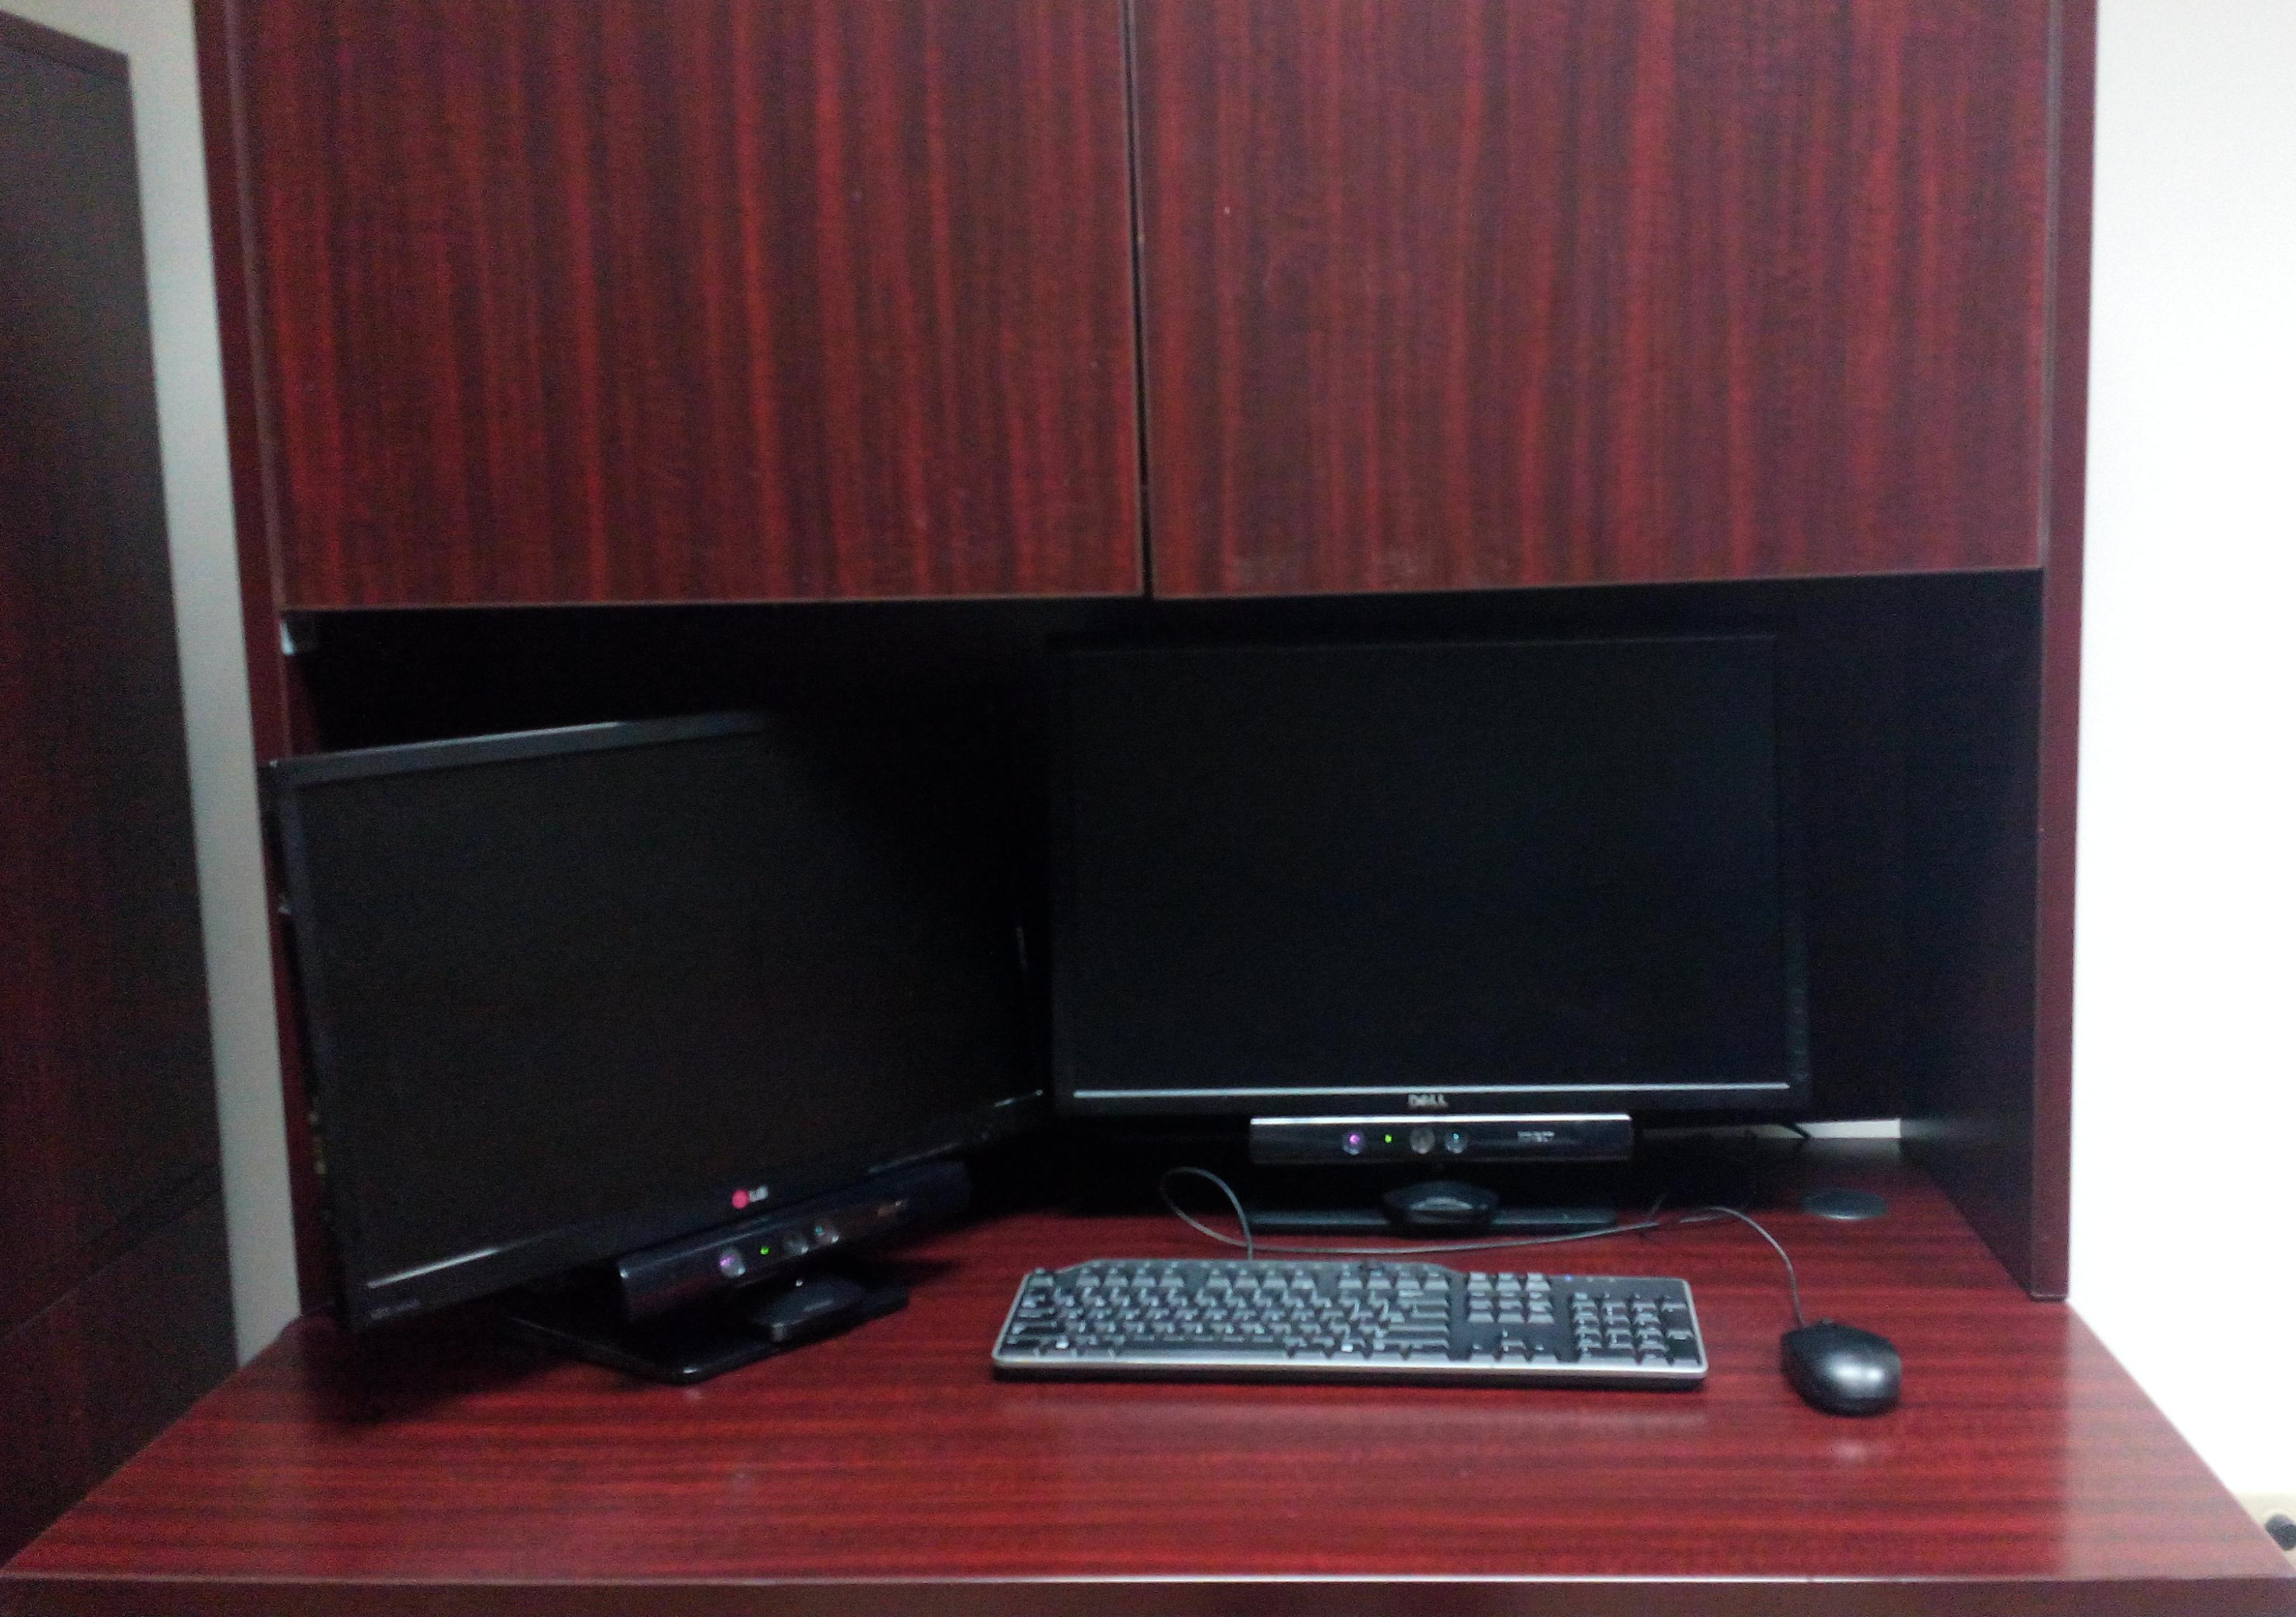
\includegraphics[scale=0.11]{./Figures/iluminacion.jpg}
\end{center}
\caption{Laboratorio en condiciones estándar de iluminación.}
\label{fig:LabIluminado}
\end{figure} 

En las siguientes tablas se muestras los resultados de la iluminación. 

\begin{tabular}{ | l | c | r | }
\hline
  1 & 2 & 3 \\
%  4 & 5 & 6 \\
%  7 & 8 & 9 \\ 
\hline
\end{tabular}


\subsection{Experimento con iluminación media} 
Para este experimento se capturaron imágenes con iluminación media, como la que se muestra en la figura . Las pruebas se realizaron con al usuario en a diferentes distintas a $70$, $80$ y $90$ $cm.$ del Kinect frontal. 

\begin{figure}[h!]
\begin{center} 
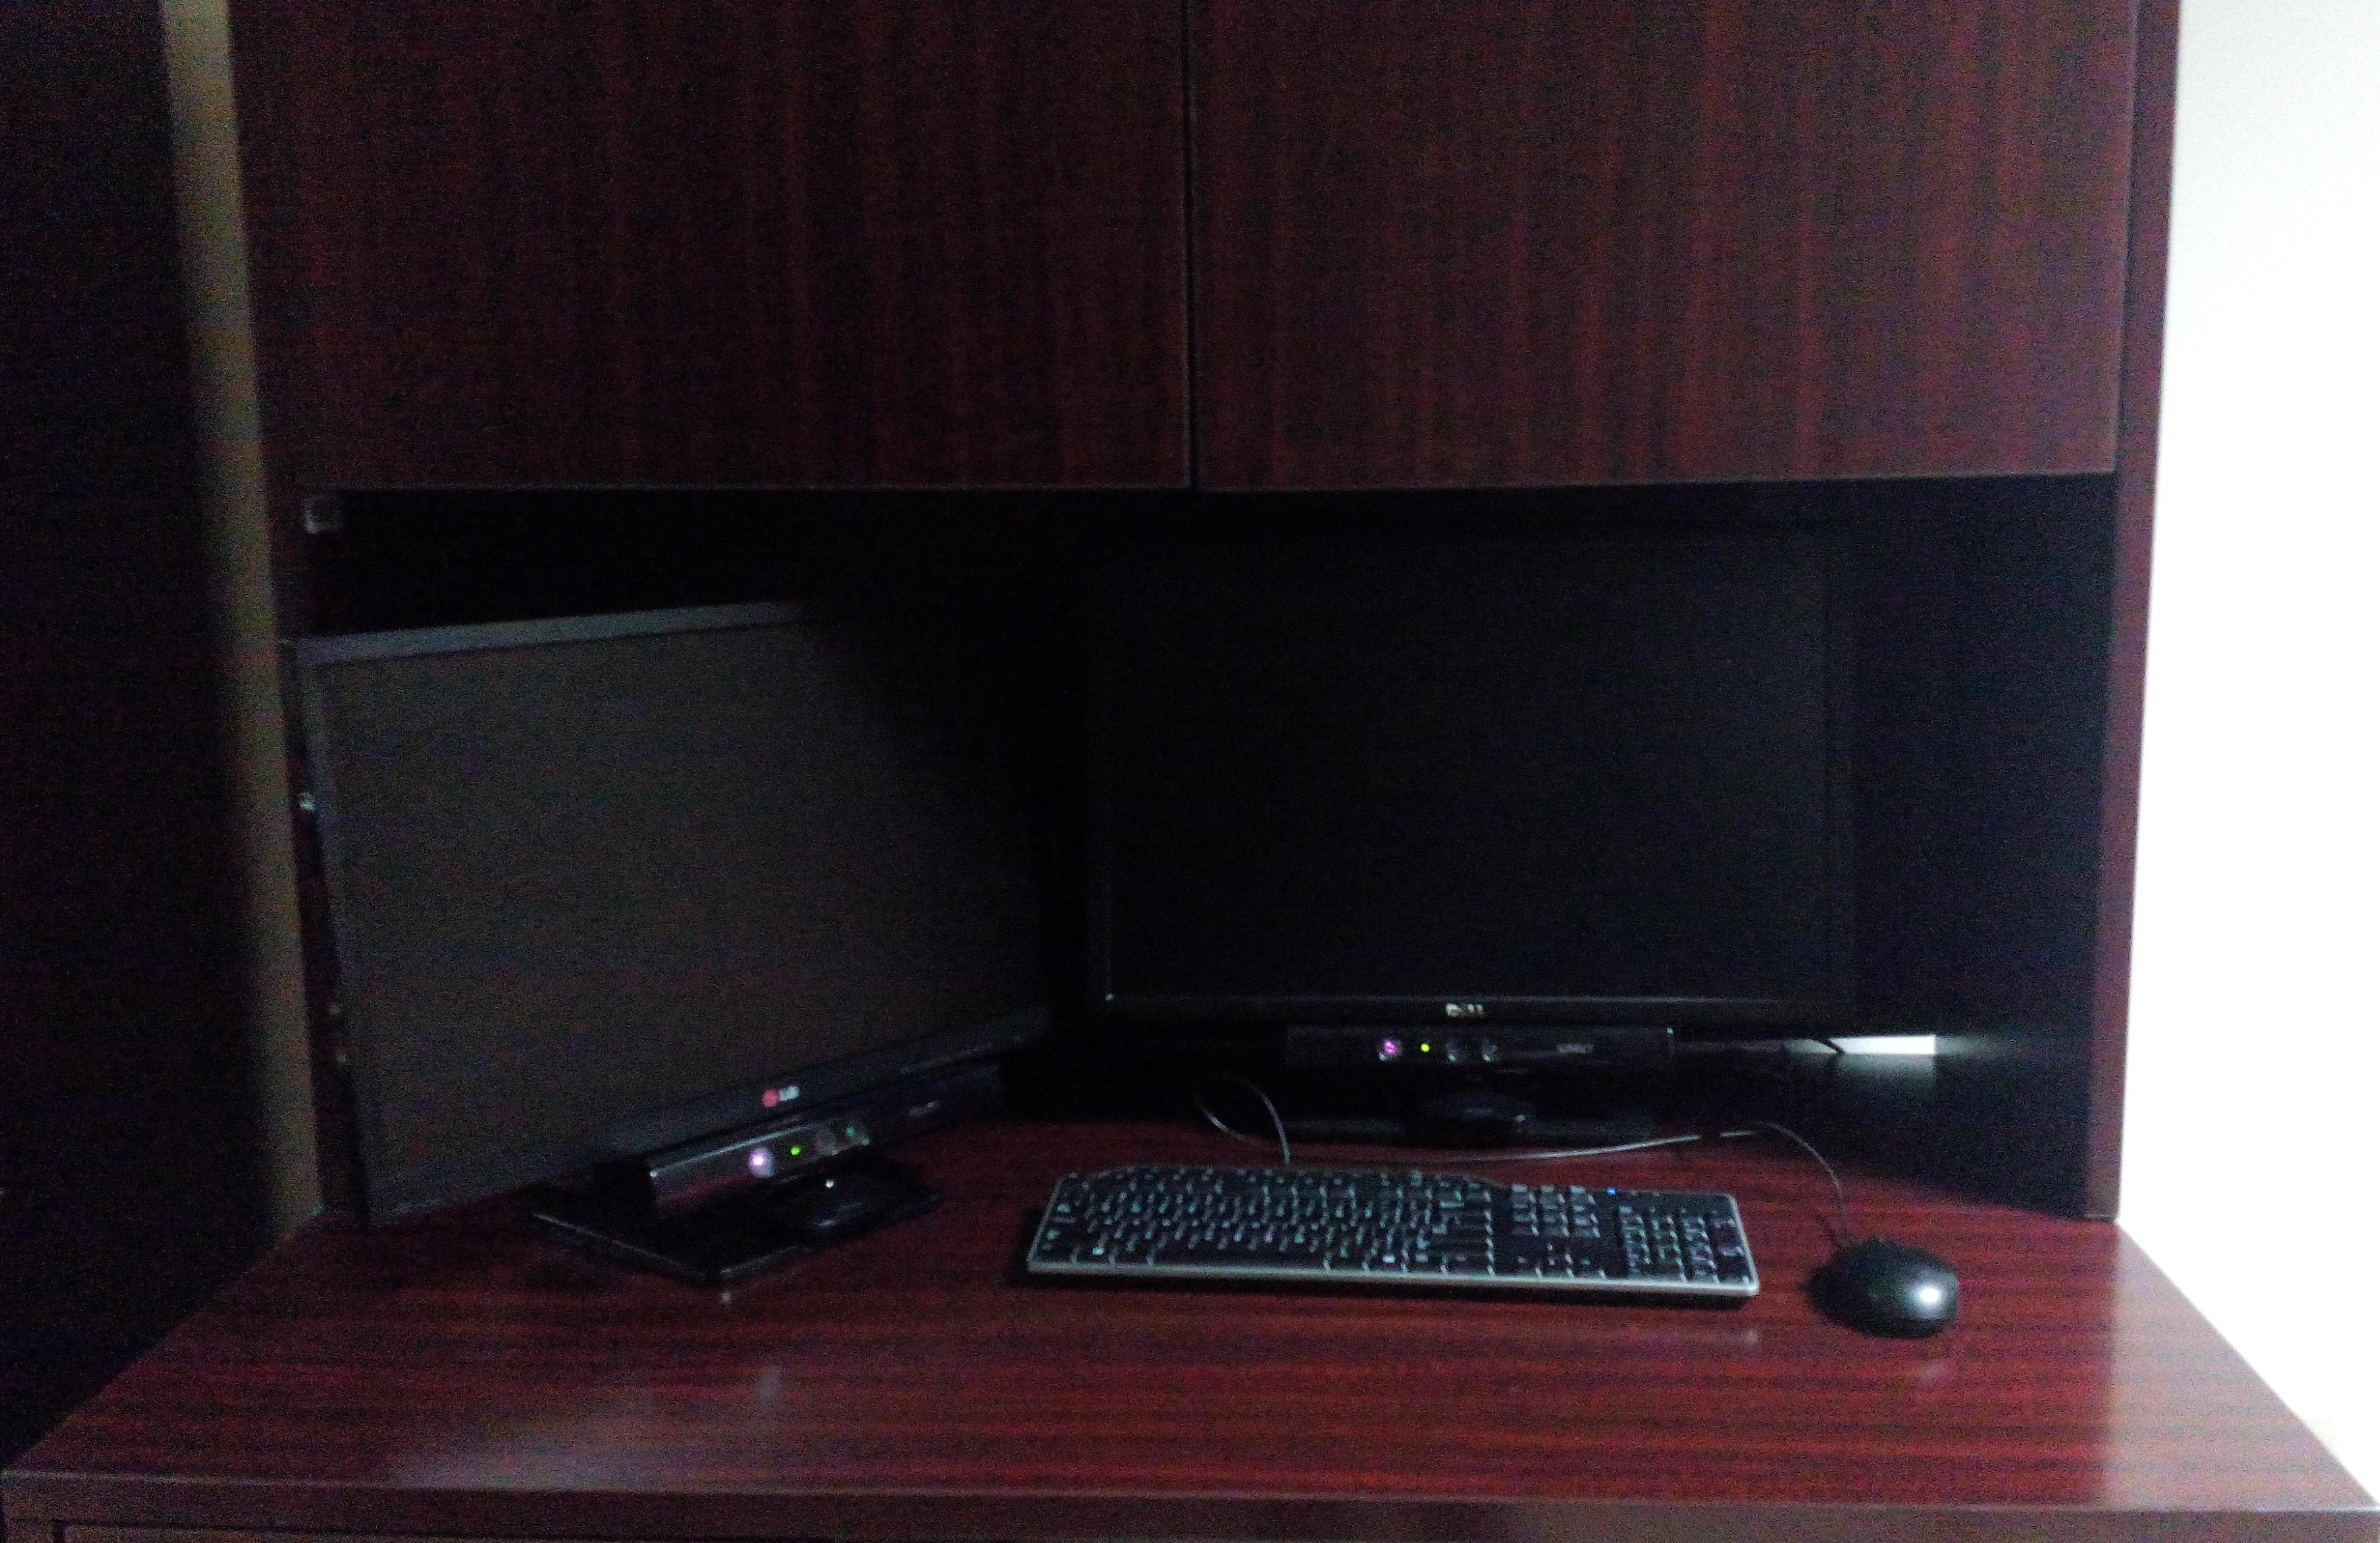
\includegraphics[scale=0.11]{./Figures/mediailuminacion.jpg}
\end{center}
\caption{Laboratorio en condiciones con iluminación media.}
\label{fig:LabMedioIluminado} 
\end{figure} 

Para este experimento se capturaron imágenes con baja iluminación, como la que se muestra en la figura . Las pruebas se realizaron con al usuario en a diferentes distintas a $70$, $80$ y $90$ $cm.$ del Kinect frontal. 

\begin{figure}[h!]
\begin{center} 
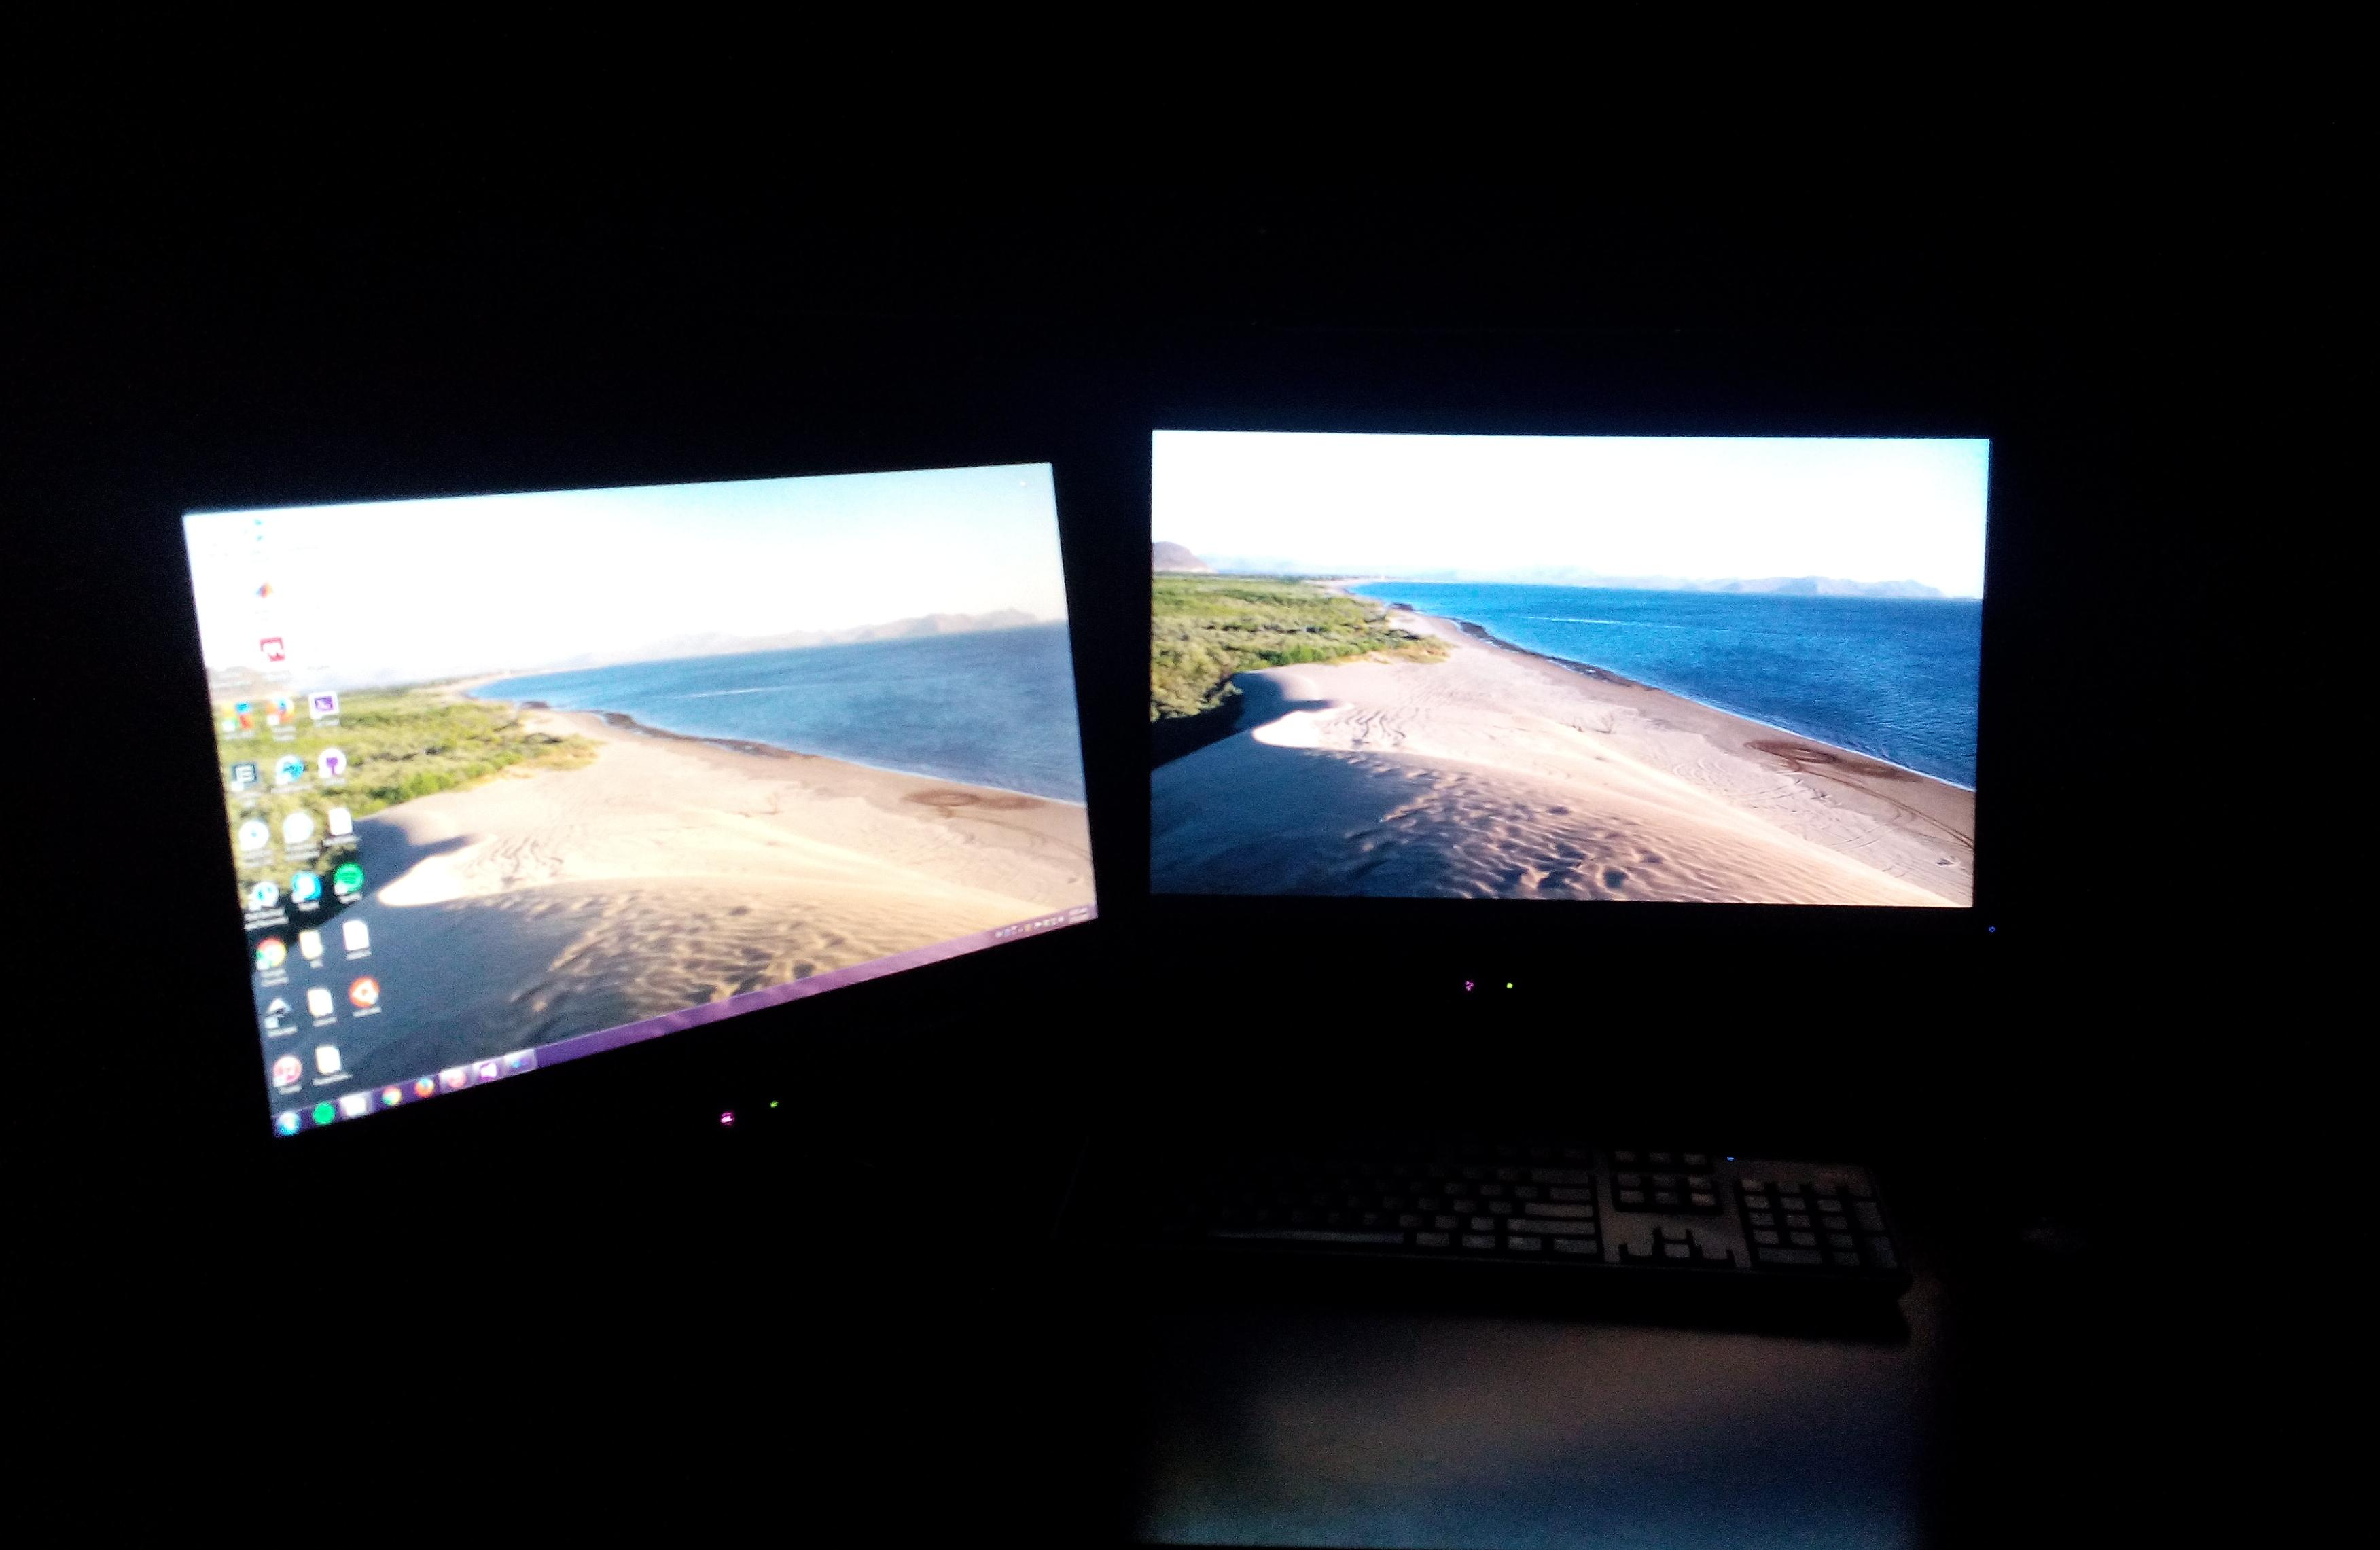
\includegraphics[scale=0.11]{./Figures/noIluminacion.jpg}
\end{center}
\caption{Laboratorio en condiciones con baja iluminación.}
\label{fig:LabNoIluminado} 
\end{figure}

%:::::::::::::::::::::::::::::::::::::::::::::::::::::::::::::::::::::::::::::::::::::::::::::::::::::::::::::::::

\section{Experimentos de gestos dinámicos}\label{TestDinamicGestures} 


%---------------------------------------------------------------------------------------------------------------------- 
\newpage
%%=====================================================
%\begin{tabular} { c c c }
% cell1 & cell2 & cell3 \\ 
% cell4 & cell5 & cell6 \\  
% cell7 & cell8 & cell9    
%\end{tabular}
%\end{center}
%
%\begin{center}[b]
%\begin{tabular}{ |c|c|c| } 
% \hline
% cell1 & cell2 & cell3 \\ 
% cell4 & cell5 & cell6 \\ 
% cell7 & cell8 & cell9 \\ 
% \hline
%\end{tabular}
%\end{center}
%
%\begin{center}[c]
% \begin{tabular}{||c c c c||} 
% \hline
% Col1 & Col2 & Col2 & Col3 \\ [0.5ex] 
% \hline\hline
% 1 & 6 & 87837 & 787 \\ 
% \hline
% 2 & 7 & 78 & 5415 \\
% \hline
% 3 & 545 & 778 & 7507 \\
% \hline
% 4 & 545 & 18744 & 7560 \\
% \hline
% 5 & 88 & 788 & 6344 \\ [1ex] 
% \hline
%\end{tabular}
%\end{center}
%
%\begin{center}[d]
%\begin{tabular}{ | b{5cm} | m{2cm}| m{2cm} | } 
%\hline
%The aligning options are m for middle, p for top and b for bottom.& cell2 & cell3 \\ 
%\hline
%cell1 dummy text dummy text dummy text & cell5 & cell6 \\ 
%\hline
%cell7 & cell8 & cell9 \\ 
%\hline
%\end{tabular}
%\end{center}
%
%\begin{center}[e]
%\begin{tabular}{ |p{3cm}||p{3cm}|p{3cm}|p{3cm}|  }
% \hline
% \multicolumn{4}{|c|}{Country List} \\
% \hline
% Country Name     or Area Name& ISO ALPHA 2 Code &ISO ALPHA 3 Code&ISO numeric Code\\
% \hline
% Afghanistan   & AF    &AFG&   004\\
% Aland Islands&   AX  & ALA   &248\\
% Albania &AL & ALB&  008\\
% Algeria    &DZ & DZA&  012\\
% American Samoa&   AS  & ASM&016\\
% Andorra& AD  & AND   &020\\
% Angola& AO  & AGO&024\\
% \hline
%\end{tabular}
%\end{center}
%\begin{center}[f]
%\begin{tabular}{ |c|c|c|c| } 
%\hline
%col1 & col2 & col3 \\
%\hline
%\multirow{3}{4em}{Multiple row} & cell2 & cell3 \\ 
%& cell5 & cell6 \\ 
%& cell8 & cell9 \\ 
%\hline
%\end{tabular}
%\end{center} 
%
%
%\begin{table}
%\footnotesize
%\centering
%\caption{Mauris et imperdiet     tortor. Maecenas consectetur lacus elit, dignissim eleifend dolor  ornare ut. Aenean euismod porta nisi, et volutpat ex laoreet sit amet. Sed ac elit vestibulum neque ultrices feugiat}
%\label{tab:recopilacionDeCuestionarios}
%%\rotatebox{90}{
%\begin{tabular}{m{0.2cm}m{2.5cm}m{2.5cm}m{2.5cm}m{2.5cm}m{2.5cm}}
%\hline\noalign{\smallskip}
% & \textbf{FFS} & \textbf{SOFA} & \textbf{FQ} & \textbf{CIS20R} & \textbf{FACIT}
%\\ \noalign{\smallskip}
%\hline
%\noalign{\smallskip}
%1	&	TAF	&	TAF	&	PF	&	PF	&	PF\\
%2	&	TAF	&	CM	&	CS	&	EE	&	PF\\
%3	&	PF	&	TAF	&	CS	&	CM	&	EE\\
%\hline
%\end{tabular}
%%}
%\end{table}